% This file was created with matplot2tikz v0.5.3.
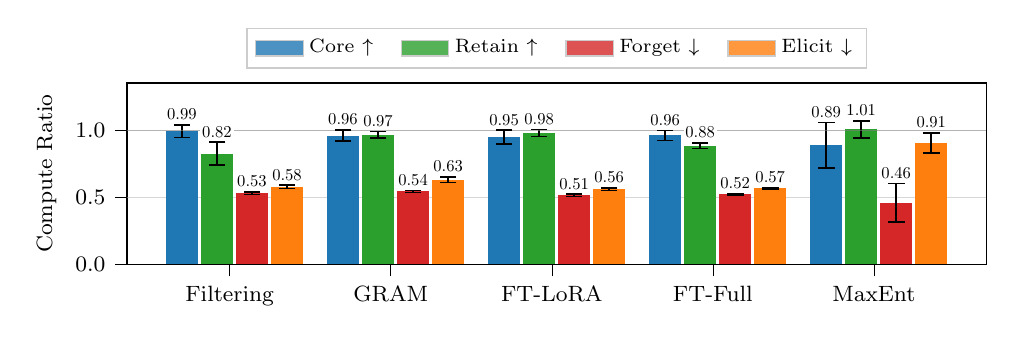
\begin{tikzpicture}

\definecolor{crimson2143940}{RGB}{214,39,40}
\definecolor{darkgray176}{RGB}{176,176,176}
\definecolor{darkorange25512714}{RGB}{255,127,14}
\definecolor{forestgreen4416044}{RGB}{44,160,44}
\definecolor{gray}{RGB}{128,128,128}
\definecolor{lightgray204}{RGB}{204,204,204}
\definecolor{steelblue31119180}{RGB}{31,119,180}

\begin{axis}[
scale only axis=true,
width=0.9\linewidth,
height=0.19\linewidth,
label style={font=\footnotesize},
tick label style={font=\footnotesize},
legend cell align={left},
legend columns=4,
legend style={
  font=\scriptsize,
  fill opacity=0.8,
  draw opacity=1,
  text opacity=1,
  at={(0.5,1.08)},
  anchor=south,
  draw=lightgray204,
  /tikz/every even column/.append style={column sep=8pt}
},
tick align=outside,
tick pos=left,
x grid style={darkgray176},
xmin=-0.6375, xmax=4.6975,
xtick style={color=black},
xtick={0,1,2,3,4},
xticklabels={Filtering,GRAM,FT-LoRA,FT-Full,MaxEnt},
xticklabel style={font=\footnotesize},
y grid style={darkgray176},
ylabel={Compute Ratio},
ymin=0, ymax=1.35,
ytick={0,0.5,1},
yticklabels={0.0,0.5,1.0},
ytick style={color=black}
]
% Faint 0.5 reference line, drawn first so it sits behind the bars.
\addplot [line width=0.28pt, darkgray176, opacity=0.5, forget plot]
table {%
-0.6375 0.5
4.6975 0.5
};
\draw[draw=none,fill=steelblue31119180] (axis cs:-0.395,0) rectangle (axis cs:-0.1975,0.991627892566709);
\addlegendimage{area legend,draw=none,fill=steelblue31119180}
\addlegendentry{Core $\uparrow$}

\draw[draw=none,fill=steelblue31119180] (axis cs:0.605,0) rectangle (axis cs:0.8025,0.958899100215159);
\draw[draw=none,fill=steelblue31119180] (axis cs:1.605,0) rectangle (axis cs:1.8025,0.947203341067582);
\draw[draw=none,fill=steelblue31119180] (axis cs:2.605,0) rectangle (axis cs:2.8025,0.96054476532688);
\draw[draw=none,fill=steelblue31119180] (axis cs:3.605,0) rectangle (axis cs:3.8025,0.886820110106901);
\draw[draw=none,fill=forestgreen4416044] (axis cs:-0.1775,0) rectangle (axis cs:0.02,0.824287820647534);
\addlegendimage{area legend,draw=none,fill=forestgreen4416044}
\addlegendentry{Retain $\uparrow$}

\draw[draw=none,fill=forestgreen4416044] (axis cs:0.8225,0) rectangle (axis cs:1.02,0.96516813682837);
\draw[draw=none,fill=forestgreen4416044] (axis cs:1.8225,0) rectangle (axis cs:2.02,0.979269485570508);
\draw[draw=none,fill=forestgreen4416044] (axis cs:2.8225,0) rectangle (axis cs:3.02,0.882959977179428);
\draw[draw=none,fill=forestgreen4416044] (axis cs:3.8225,0) rectangle (axis cs:4.02,1.00560314378137);
\draw[draw=none,fill=crimson2143940] (axis cs:0.04,0) rectangle (axis cs:0.2375,0.529996501592815);
\addlegendimage{area legend,draw=none,fill=crimson2143940}
\addlegendentry{Forget $\downarrow$}

\draw[draw=none,fill=crimson2143940] (axis cs:1.04,0) rectangle (axis cs:1.2375,0.54342366161624);
\draw[draw=none,fill=crimson2143940] (axis cs:2.04,0) rectangle (axis cs:2.2375,0.514052705600195);
\draw[draw=none,fill=crimson2143940] (axis cs:3.04,0) rectangle (axis cs:3.2375,0.520618877066234);
\draw[draw=none,fill=crimson2143940] (axis cs:4.04,0) rectangle (axis cs:4.2375,0.458490687884046);
\draw[draw=none,fill=darkorange25512714] (axis cs:0.2575,0) rectangle (axis cs:0.455,0.577964125301141);
\addlegendimage{area legend,draw=none,fill=darkorange25512714}
\addlegendentry{Elicit $\downarrow$}

\draw[draw=none,fill=darkorange25512714] (axis cs:1.2575,0) rectangle (axis cs:1.455,0.630227557277706);
\draw[draw=none,fill=darkorange25512714] (axis cs:2.2575,0) rectangle (axis cs:2.455,0.559611214747933);
\draw[draw=none,fill=darkorange25512714] (axis cs:3.2575,0) rectangle (axis cs:3.455,0.565765565716319);
\draw[draw=none,fill=darkorange25512714] (axis cs:4.2575,0) rectangle (axis cs:4.455,0.90555651905828);
\path [draw=black, semithick]
(axis cs:-0.29625,0.944555028554978)
--(axis cs:-0.29625,1.03870075657844);

\path [draw=black, semithick]
(axis cs:0.70375,0.916688545750057)
--(axis cs:0.70375,1.00110965468026);

\path [draw=black, semithick]
(axis cs:1.70375,0.894800484810594)
--(axis cs:1.70375,0.99960619732457);

\path [draw=black, semithick]
(axis cs:2.70375,0.923576102537636)
--(axis cs:2.70375,0.997513428116124);

\path [draw=black, semithick]
(axis cs:3.70375,0.718327218220626)
--(axis cs:3.70375,1.05531300199318);

\addplot [semithick, steelblue31119180, mark=-, mark size=3, mark options={solid,draw=black}, only marks]
table {%
-0.29625 0.944555028554978
0.70375 0.916688545750057
1.70375 0.894800484810594
2.70375 0.923576102537636
3.70375 0.718327218220626
};
\addplot [semithick, steelblue31119180, mark=-, mark size=3, mark options={solid,draw=black}, only marks]
table {%
-0.29625 1.03870075657844
0.70375 1.00110965468026
1.70375 0.99960619732457
2.70375 0.997513428116124
3.70375 1.05531300199318
};
\path [draw=black, semithick]
(axis cs:-0.07875,0.739198470148385)
--(axis cs:-0.07875,0.909377171146683);

\path [draw=black, semithick]
(axis cs:0.92125,0.941201033728518)
--(axis cs:0.92125,0.989135239928223);

\path [draw=black, semithick]
(axis cs:1.92125,0.953100477894393)
--(axis cs:1.92125,1.00543849324662);

\path [draw=black, semithick]
(axis cs:2.92125,0.862446026491702)
--(axis cs:2.92125,0.903473927867153);

\path [draw=black, semithick]
(axis cs:3.92125,0.942531364147202)
--(axis cs:3.92125,1.06867492341553);

\addplot [semithick, steelblue31119180, mark=-, mark size=3, mark options={solid,draw=black}, only marks]
table {%
-0.07875 0.739198470148385
0.92125 0.941201033728518
1.92125 0.953100477894393
2.92125 0.862446026491702
3.92125 0.942531364147202
};
\addplot [semithick, steelblue31119180, mark=-, mark size=3, mark options={solid,draw=black}, only marks]
table {%
-0.07875 0.909377171146683
0.92125 0.989135239928223
1.92125 1.00543849324662
2.92125 0.903473927867153
3.92125 1.06867492341553
};
\path [draw=black, semithick]
(axis cs:0.13875,0.521029247245715)
--(axis cs:0.13875,0.538963755939916);

\path [draw=black, semithick]
(axis cs:1.13875,0.535985692452006)
--(axis cs:1.13875,0.550861630780473);

\path [draw=black, semithick]
(axis cs:2.13875,0.504683105502085)
--(axis cs:2.13875,0.523422305698304);

\path [draw=black, semithick]
(axis cs:3.13875,0.515583868322294)
--(axis cs:3.13875,0.525653885810174);

\path [draw=black, semithick]
(axis cs:4.13875,0.313794849258932)
--(axis cs:4.13875,0.603186526509159);

\addplot [semithick, steelblue31119180, mark=-, mark size=3, mark options={solid,draw=black}, only marks]
table {%
0.13875 0.521029247245715
1.13875 0.535985692452006
2.13875 0.504683105502085
3.13875 0.515583868322294
4.13875 0.313794849258932
};
\addplot [semithick, steelblue31119180, mark=-, mark size=3, mark options={solid,draw=black}, only marks]
table {%
0.13875 0.538963755939916
1.13875 0.550861630780473
2.13875 0.523422305698304
3.13875 0.525653885810174
4.13875 0.603186526509159
};
\path [draw=black, semithick]
(axis cs:0.35625,0.566305050965915)
--(axis cs:0.35625,0.589623199636366);

\path [draw=black, semithick]
(axis cs:1.35625,0.609607759042544)
--(axis cs:1.35625,0.650847355512868);

\path [draw=black, semithick]
(axis cs:2.35625,0.550167691828637)
--(axis cs:2.35625,0.569054737667228);

\path [draw=black, semithick]
(axis cs:3.35625,0.560063441543313)
--(axis cs:3.35625,0.571467689889324);

\path [draw=black, semithick]
(axis cs:4.35625,0.830823547426428)
--(axis cs:4.35625,0.980289490690132);

\addplot [semithick, steelblue31119180, mark=-, mark size=3, mark options={solid,draw=black}, only marks]
table {%
0.35625 0.566305050965915
1.35625 0.609607759042544
2.35625 0.550167691828637
3.35625 0.560063441543313
4.35625 0.830823547426428
};
\addplot [semithick, steelblue31119180, mark=-, mark size=3, mark options={solid,draw=black}, only marks]
table {%
0.35625 0.589623199636366
1.35625 0.650847355512868
2.35625 0.569054737667228
3.35625 0.571467689889324
4.35625 0.980289490690132
};
\addplot [line width=0.28pt, gray, opacity=0.6, forget plot]
table {%
-0.6375 1
4.6975 1
};
\draw (axis cs:-0.29625,1.05949174903098) node[
  scale=0.6,
  fill=white,
  draw=none,
  line width=0.4pt,
  inner sep=1.1pt,
  fill opacity=1,
  anchor=south,
  text=black,
  rotate=0.0
]{0.99};
\draw (axis cs:0.70375,1.0219006471328) node[
  scale=0.6,
  fill=white,
  draw=none,
  line width=0.4pt,
  inner sep=1.1pt,
  fill opacity=1,
  anchor=south,
  text=black,
  rotate=0.0
]{0.96};
\draw (axis cs:1.70375,1.02039718977711) node[
  scale=0.6,
  fill=white,
  draw=none,
  line width=0.4pt,
  inner sep=1.1pt,
  fill opacity=1,
  anchor=south,
  text=black,
  rotate=0.0
]{0.95};
\draw (axis cs:2.70375,1.01951342811612) node[
  scale=0.6,
  fill=white,
  draw=none,
  line width=0.4pt,
  inner sep=1.1pt,
  fill opacity=1,
  anchor=south,
  text=black,
  rotate=0.0
]{0.96};
\draw (axis cs:3.70375,1.07610399444571) node[
  scale=0.6,
  fill=white,
  draw=none,
  line width=0.4pt,
  inner sep=1.1pt,
  fill opacity=1,
  anchor=south,
  text=black,
  rotate=0.0
]{0.89};
\draw (axis cs:-0.07875,0.931141657946251) node[
  scale=0.6,
  fill=white,
  draw=none,
  line width=0.4pt,
  inner sep=1.1pt,
  fill opacity=1,
  anchor=south,
  text=black,
  rotate=0.0
]{0.82};
\draw (axis cs:0.92125,1.01089972672779) node[
  scale=0.6,
  fill=white,
  draw=none,
  line width=0.4pt,
  inner sep=1.1pt,
  fill opacity=1,
  anchor=south,
  text=black,
  rotate=0.0
]{0.97};
\draw (axis cs:1.92125,1.02720298004619) node[
  scale=0.6,
  fill=white,
  draw=none,
  line width=0.4pt,
  inner sep=1.1pt,
  fill opacity=1,
  anchor=south,
  text=black,
  rotate=0.0
]{0.98};
\draw (axis cs:2.92125,0.925473927867153) node[
  scale=0.6,
  fill=white,
  draw=none,
  line width=0.4pt,
  inner sep=1.1pt,
  fill opacity=1,
  anchor=south,
  text=black,
  rotate=0.0
]{0.88};
\draw (axis cs:3.92125,1.0904394102151) node[
  scale=0.6,
  fill=white,
  draw=none,
  line width=0.4pt,
  inner sep=1.1pt,
  fill opacity=1,
  anchor=south,
  text=black,
  rotate=0.0
]{1.01};
\draw (axis cs:0.13875,0.560728242739485) node[
  scale=0.6,
  fill=white,
  draw=none,
  line width=0.4pt,
  inner sep=1.1pt,
  fill opacity=1,
  anchor=south,
  text=black,
  rotate=0.0
]{0.53};
\draw (axis cs:1.13875,0.572626117580041) node[
  scale=0.6,
  fill=white,
  draw=none,
  line width=0.4pt,
  inner sep=1.1pt,
  fill opacity=1,
  anchor=south,
  text=black,
  rotate=0.0
]{0.54};
\draw (axis cs:2.13875,0.545186792497872) node[
  scale=0.6,
  fill=white,
  draw=none,
  line width=0.4pt,
  inner sep=1.1pt,
  fill opacity=1,
  anchor=south,
  text=black,
  rotate=0.0
]{0.51};
\draw (axis cs:3.13875,0.547653885810174) node[
  scale=0.6,
  fill=white,
  draw=none,
  line width=0.4pt,
  inner sep=1.1pt,
  fill opacity=1,
  anchor=south,
  text=black,
  rotate=0.0
]{0.52};
\draw (axis cs:4.13875,0.624951013308727) node[
  scale=0.6,
  fill=white,
  draw=none,
  line width=0.4pt,
  inner sep=1.1pt,
  fill opacity=1,
  anchor=south,
  text=black,
  rotate=0.0
]{0.46};
\draw (axis cs:0.35625,0.611387686435935) node[
  scale=0.6,
  fill=white,
  draw=none,
  line width=0.4pt,
  inner sep=1.1pt,
  fill opacity=1,
  anchor=south,
  text=black,
  rotate=0.0
]{0.58};
\draw (axis cs:1.35625,0.672611842312436) node[
  scale=0.6,
  fill=white,
  draw=none,
  line width=0.4pt,
  inner sep=1.1pt,
  fill opacity=1,
  anchor=south,
  text=black,
  rotate=0.0
]{0.63};
\draw (axis cs:2.35625,0.590819224466796) node[
  scale=0.6,
  fill=white,
  draw=none,
  line width=0.4pt,
  inner sep=1.1pt,
  fill opacity=1,
  anchor=south,
  text=black,
  rotate=0.0
]{0.56};
\draw (axis cs:3.35625,0.593467689889324) node[
  scale=0.6,
  fill=white,
  draw=none,
  line width=0.4pt,
  inner sep=1.1pt,
  fill opacity=1,
  anchor=south,
  text=black,
  rotate=0.0
]{0.57};
\draw (axis cs:4.35625,1.0020539774897) node[
  scale=0.6,
  fill=white,
  draw=none,
  line width=0.4pt,
  inner sep=1.1pt,
  fill opacity=1,
  anchor=south,
  text=black,
  rotate=0.0
]{0.91};
\end{axis}

\end{tikzpicture}
